
%(BEGIN_QUESTION)
% Copyright 2012, Tony R. Kuphaldt, released under the Creative Commons Attribution License (v 1.0)
% This means you may do almost anything with this work of mine, so long as you give me proper credit

Geometry may be used to elegantly prove the Pythagorean Theorem.  Shown here are two squares of equal area, each with four right triangles embedded within, occupying area of their own:

$$\includegraphics[width=15.5cm]{i02677x01.eps}$$

Explain how these two figures prove the Pythagorean Theorem, where $a^2 + b^2 = c^2$.

\underbar{file i02677}
%(END_QUESTION)





%(BEGIN_ANSWER)

In both squares, the total area is equal because the squares have identical dimensions.  In both squares, the area occupied by the four triangles is also equal, because the triangles all share the same dimensions.  Therefore, the total shaded area in each square must also be equal.

\vskip 10pt

As you can see, the left square's shaded area is equal to $c^2$, while the right square's shaded area is equal to the sum of $a^2 + b^2$, thereby proving the Pythagorean Theorem.

%(END_ANSWER)





%(BEGIN_NOTES)


%INDEX% Mathematics review: trigonometric calculations

%(END_NOTES)


